\documentclass[handout,nooutcomes,noauthor]{ximera}

\author{Bart Snapp}

\input{../../../preamble.tex}

\title[Collaborate:]{Describing regions}

\begin{document}
\begin{abstract}
  We describe areas and volumes of regions using iterated integrals.
\end{abstract}
\maketitle

\textbf{Work in groups of 3--4, writing your answers on a separate
  sheet of paper.}

\section{Trivial regions}


\begin{problem}
  Without doing \textbf{any} integrals, evaluate
  \[
  \iint_R \d A
  \]
  where
  \[
  R =\{(x,y):-2\le x\le 4 \text{ and } -6\le y\le 1\}.
  \]
\end{problem}


\begin{problem}
  Without doing \textbf{any} integrals, evaluate
  \[
  \iiint_R \d V
  \]
  where
  \[
  R =\{(x,y,z):-4\le x\le 3, 
    -1\le y\le 5,\text{ and, } -3\le z\le 2\}.
  \]
\end{problem}

\section{Two-dimensional regions}

\begin{problem}
  Consider the region
  \[
  R=\{(x,y):0\le x\le 2+\cos(y)\text{ and }0<y<2\pi\}
  \]
  \begin{image}[1.75in]
    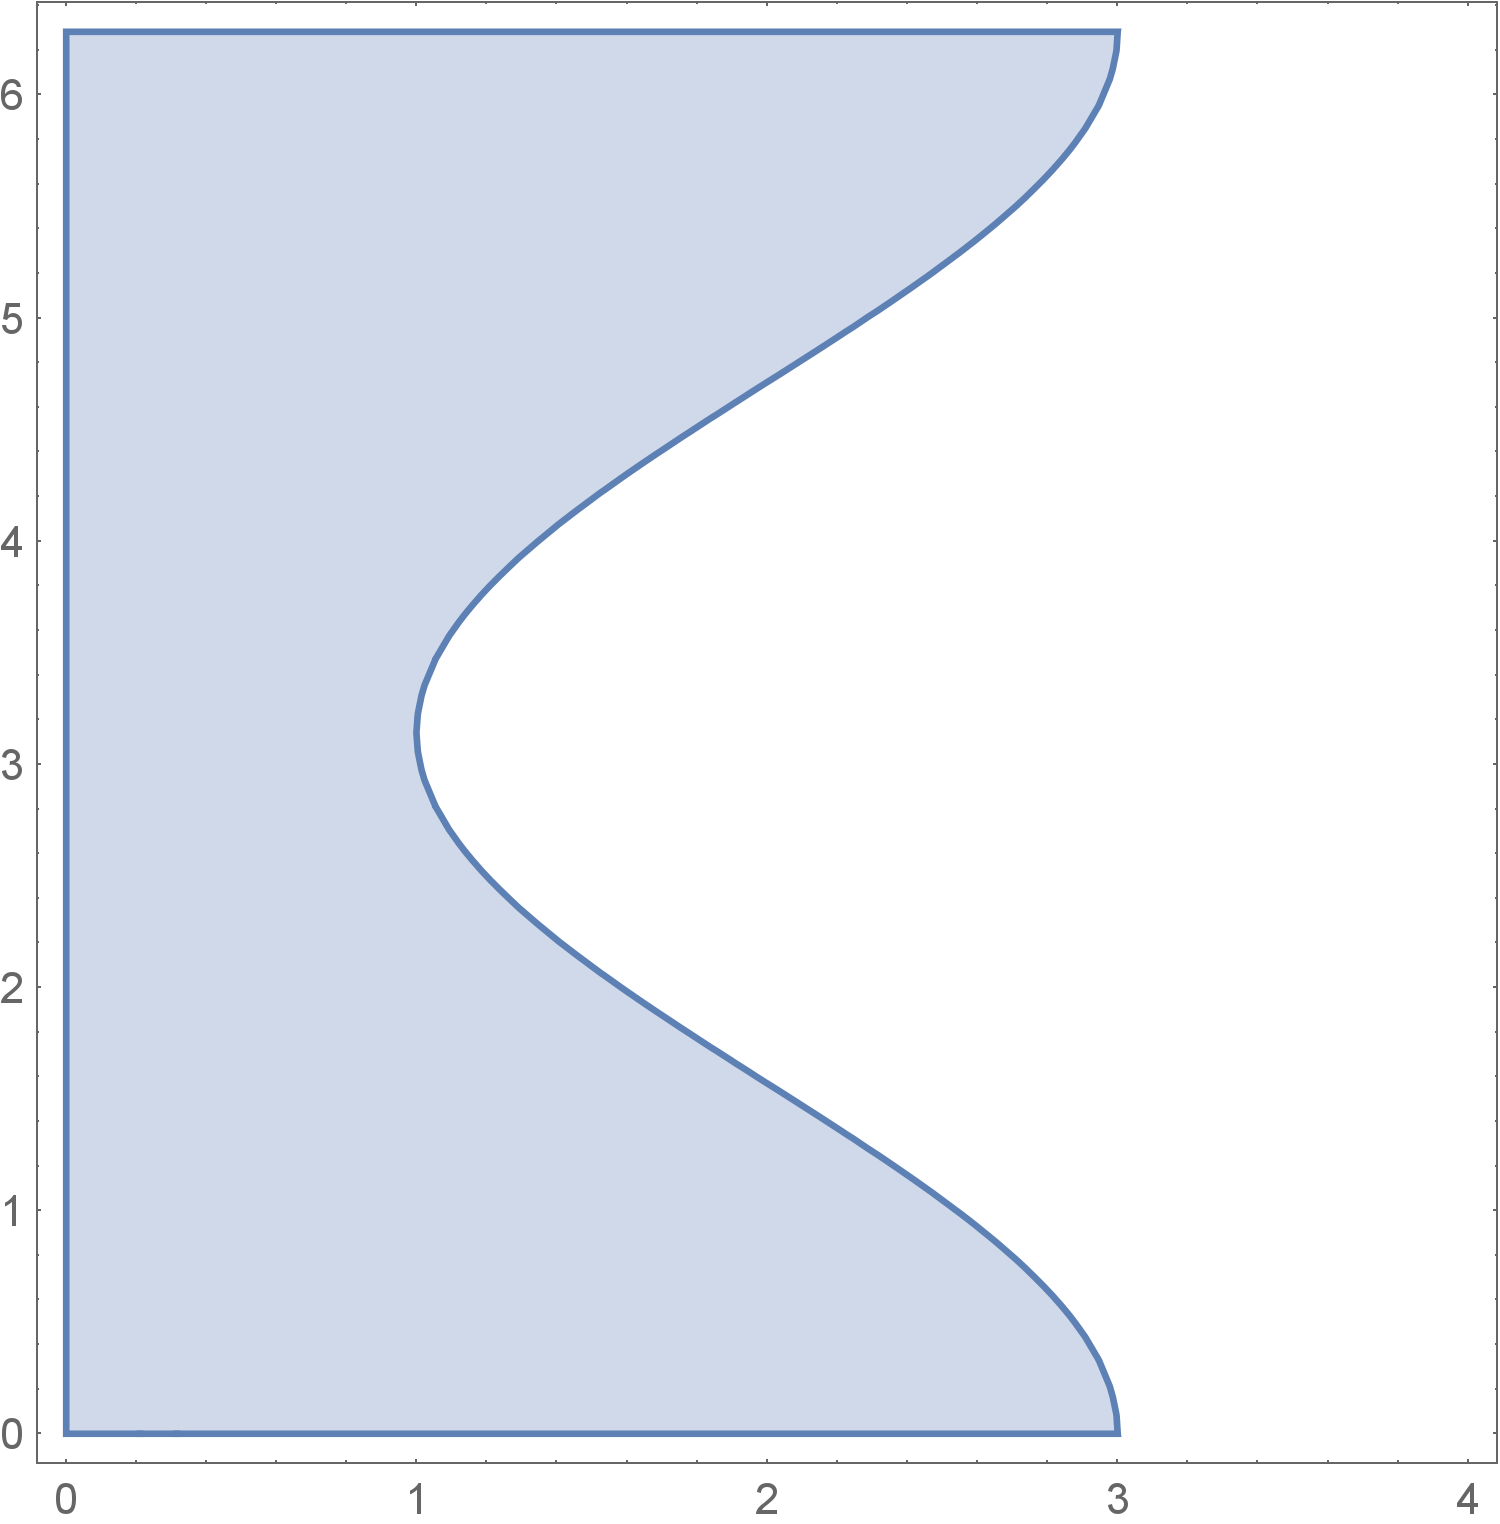
\includegraphics{region.png}
  \end{image}
  Compute the area of this region with an iterated integral where one
  integrates first with respect to $x$ and next integrates with
  respect to $y$.
  
  \textbf{As a challenge}, compute the area with an iterated integral
  where one integrates first with respect to $y$ and next integrates
  with respect to $x$.
\end{problem}


\begin{problem}
  Consider the region
   \begin{image}[2.5in]
    \begin{tikzpicture}
      \begin{axis}[
          tick label style={font=\scriptsize},
          axis y line=middle,axis x line=middle,
          name=myplot,
	  xtick={-1.5,-1,...,1.5},
	  ytick={-1.5,-1,...,1.5},
          grid = major,
          ymin=-1.5,ymax=1.5,%
	  xmin=-1.5,xmax=1.5,
          rounded corners=.5pt
        ]
        \draw [ultra thick,fill=fill1,draw=penColor] (axis cs: 0,-1) -- (axis cs: 1,1)-- (axis cs: -1,1)  -- cycle;
        
      \end{axis}
      
      \node [right] at (myplot.right of origin) {\scriptsize $x$};
      \node [above] at (myplot.above origin) {\scriptsize $y$};
    \end{tikzpicture}
   \end{image}
   \begin{enumerate}
   \item Compute the area of this region with an iterated integral
     where one integrates first with respect to $y$ and next
     integrates with respect to $x$.
   \item Compute the area of this region with an iterated integral
     where one integrates first with respect to $x$ and next
     integrates with respect to $y$.
   \end{enumerate}
\end{problem}

\begin{problem}
  Consider the ellipse centered at the origin:
  \begin{image}[2in]
    \begin{tikzpicture}
      \begin{axis}[
          tick label style={font=\scriptsize},
          axis y line=middle,axis x line=middle,
          name=myplot,axis on top,
	  xtick={-4,-3,...,4},
	  ytick={-1.5,-1,...,1.5},
          %grid = major,
          ymin=-1.5,ymax=1.5,%
	  xmin=-4.5,xmax=4.5,
          rounded corners=.5pt
        ]
        \addplot[penColor, fill= fill1,ultra thick,domain=0:360,samples=200] ({4*cos(x)},{1*sin(x)});
        
        
      \end{axis}
      
      \node [right] at (myplot.right of origin) {\scriptsize $x$};
      \node [above] at (myplot.above origin) {\scriptsize $y$};
    \end{tikzpicture}
  \end{image}
  Recall that the implicit formula for an ellipse is given by
  \[
  \left(\frac{x-x_0}{a}\right)^2 + \left(\frac{y-y_0}{b}\right)^2 = 1.
  \]
  \begin{enumerate}
   \item Compute the area of this region with an iterated integral
     where one integrates first with respect to $y$ and next
     integrates with respect to $x$.
   \item Compute the area of this region with an iterated integral
     where one integrates first with respect to $x$ and next
     integrates with respect to $y$.
   \end{enumerate}
\end{problem}

\begin{problem}
  Consider the following region:
  \begin{image}[2in]
    \begin{tikzpicture}
      \begin{axis}[
          tick label style={font=\scriptsize},
          axis y line=middle,axis x line=middle,
          name=myplot,axis on top,
	  xtick={-1.5,-1,...,1.5},
	  ytick={-.5,0,...,1.5},
          %grid = major,
          ymin=-.5,ymax=1.5,%
	  xmin=-1.5,xmax=1.5,
          rounded corners=.5pt
        ]
        \addplot[draw=none, fill= fill1,domain=-1:1] {1}\closedcycle;
        \addplot[penColor, fill= fill1,ultra thick,domain=45:135] ({(sqrt(2)) * cos(x)},{(sqrt(2))*sin(x)});
        \addplot[draw=none, fill= white,ultra thick,domain=0:1] {x}\closedcycle;
        \addplot[draw=none, fill=white,ultra thick,domain=-1:0] {-x}\closedcycle;

        \addplot[mark=*,penColor] coordinates {(1,1)};

        \addplot[penColor,ultra thick,domain=0:1] {x};
        \addplot[penColor,ultra thick,domain=-1:0] {-x};

        \node [right] at (axis cs: 1,1) {$(1,1)$};
        
      \end{axis}
      
      \node [right] at (myplot.right of origin) {\scriptsize $x$};
      \node [above] at (myplot.above origin) {\scriptsize $y$};
    \end{tikzpicture}
  \end{image}
  The largest $y$-value of the region is $y=\sqrt{2}$. 
  \begin{enumerate}
  \item Compute the area of this region with an iterated integral
    where one integrates first with respect to $y$ and next integrates
    with respect to $x$.
  \item Compute the area of this region with an iterated integral
    where one integrates first with respect to $x$ and next integrates
    with respect to $y$.
  \end{enumerate}
\end{problem}




\section{Three-dimensional regions}


\begin{problem}
  Consider the region bounded by the planes:
  \begin{itemize}
  \item $x=0$
  \item $y=0$
  \item $z=0$
  \item $6x+3y+2z = 24$
  \end{itemize}
  Sketch this region and set-up \textbf{six} iterated integrals that
  compute the volume of this solid, all which integrate in a different
  order.
\end{problem}


\begin{problem}
  Consider the region:
  \[
  R=\{(x,y,z): 0 \le x \le 1, -1\le y \le 0, 0\le z\le y^2\}
  \]
  \begin{image}[2in]
    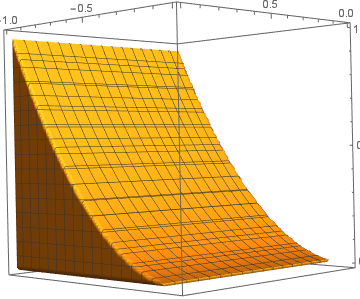
\includegraphics{threeRegion2.png}
  \end{image}
  Set up \textbf{six} iterated integrals that compute the volume of this solid,
  all which integrate in a different order.
\end{problem}

\begin{problem}
  Consider the region:
  \[
  R=\{(x,y,z): 0 \le x \le 1, \sqrt{x}\le y \le 1, 0\le z\le 1-y\}
  \]
  \begin{image}[2in]
    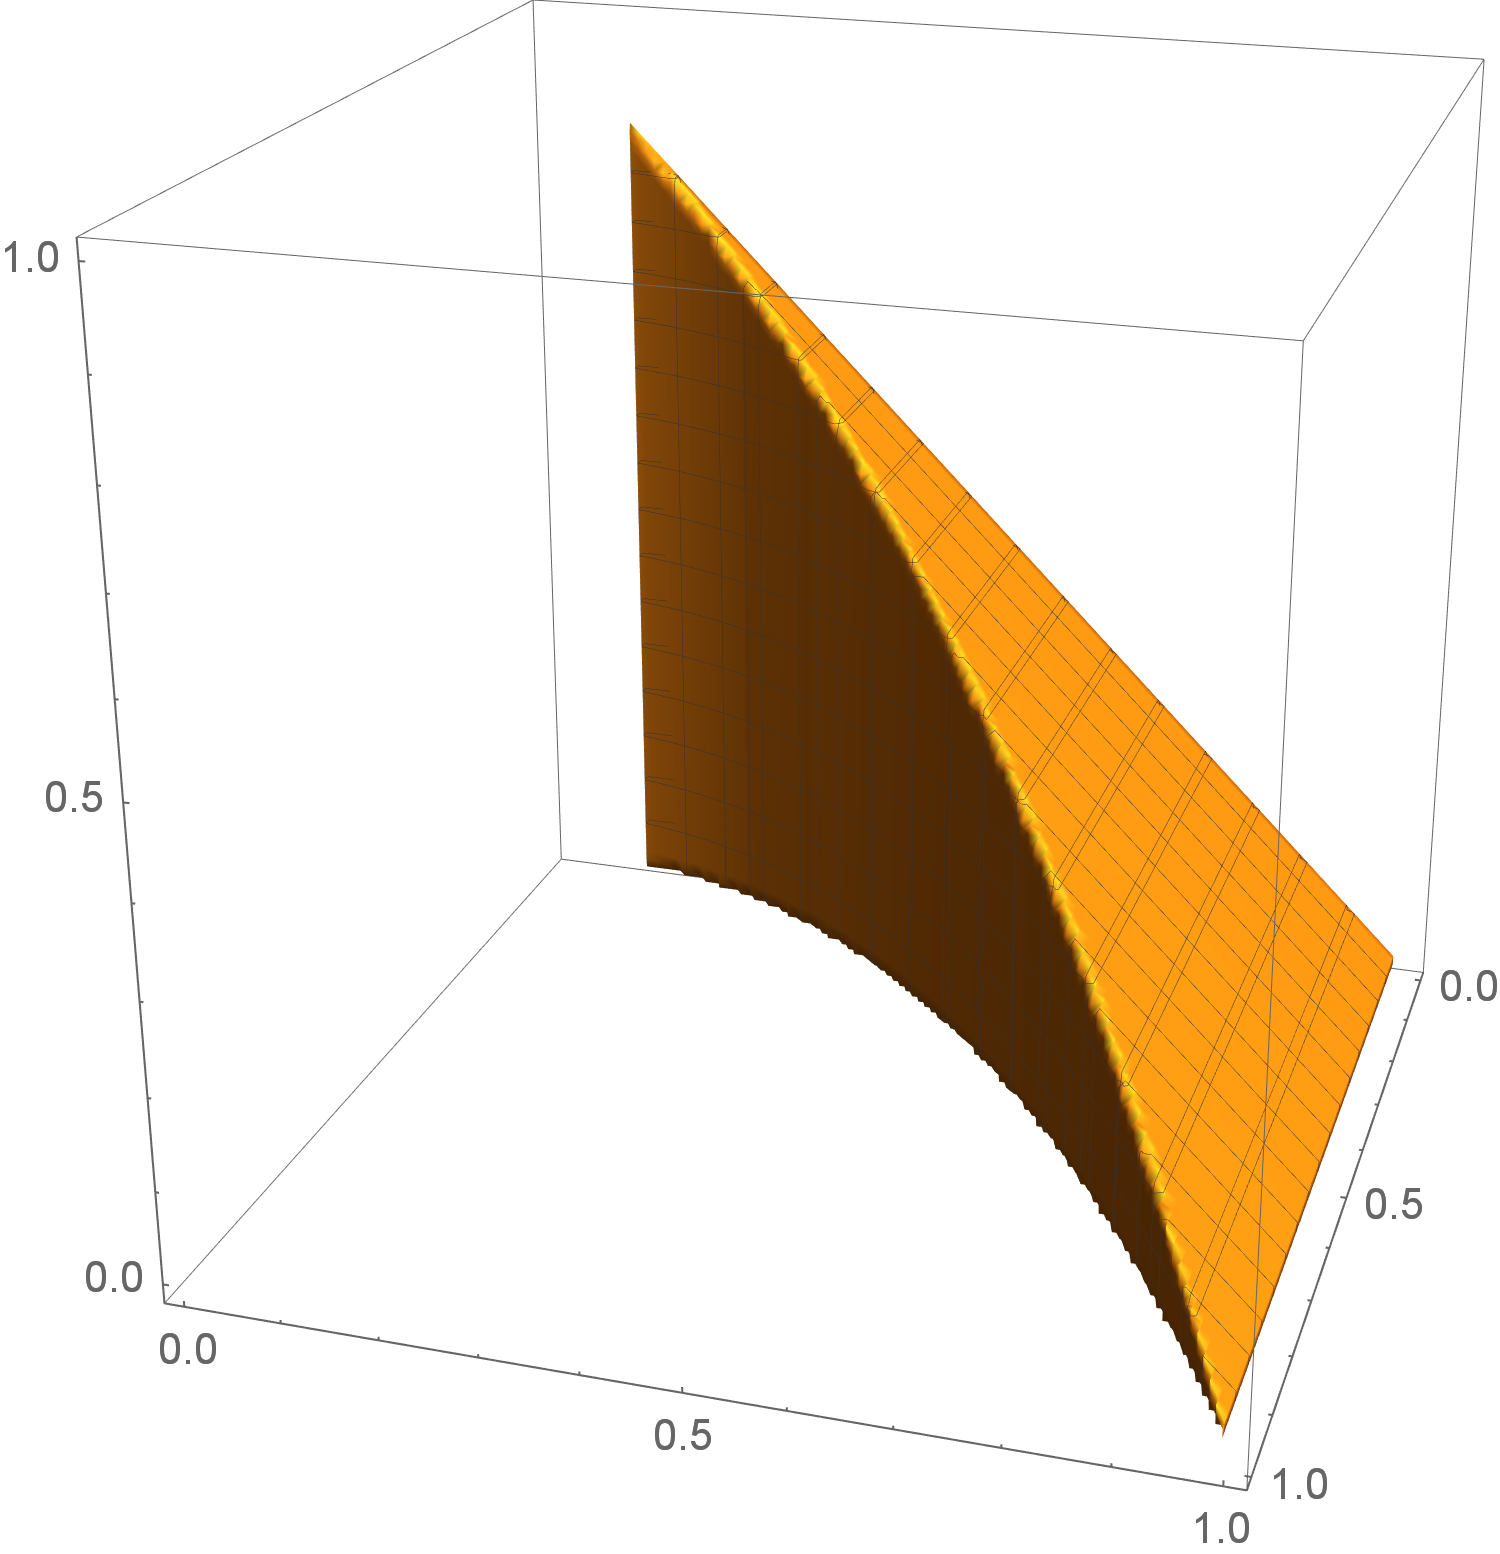
\includegraphics{threeRegion1.png}
  \end{image}
  Set up \textbf{six} iterated integrals that compute the volume of this solid,
  all which integrate in a different order.
\end{problem}


\end{document}
